\chapter{Visualizing Dynamic Input Graphs}
\label{chap:visualizing-dynamic-input-graphs}

Extending the approach discussed in the previous section to dynamic input graphs is challenging primarily because we must try to preserve the viewer's mental map as the underlying data changes over time. We want the visualization at different points in time to be similar enough so that the viewer can clearly tell what parts have changed \cite{mashima2011visualizing}, yet allow for the required changes in geography and topology. Still, changes between visualizations of consecutive points in time should minimize movement and allow for smooth animations therebetween.

The pipeline for static inputs discussed in the previous section does not satisfy these requirements. Running through the entire pipeline with a different, albeit similar, input graph, may result in a completely different visualization: The filtering \& embedding and transformation phases in particular have way too many degrees of freedom in choosing which edges to visualize, how to combinatorially embed the graph, and how to geometrically embed the boundary graph. We therefore extend the pipeline in a way that allows for small, incremental updates to be propagated through the individual phases. A rough sketch of the extended pipeline is depicted in \cref{fig:dynamic-pipeline}.

%Note that the final visualization phase does not need to be adjusted for the dynamic case, the implementation from the static case can be reused without any modifications.

\begin{figure}[H]
	\centering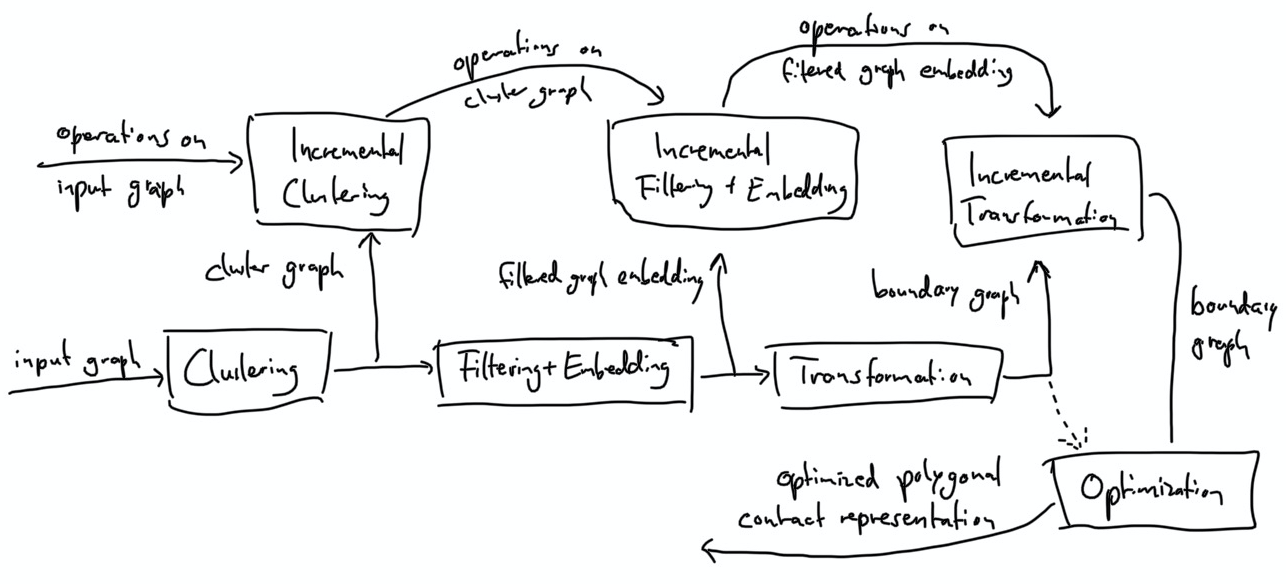
\includegraphics[width=0.9\textwidth]{Resources/DynamicPipeline.png}
	\caption{Overview of the algorithmic pipeline for dynamic input graphs.}
	\label{fig:dynamic-pipeline}
\end{figure}

\todo{Explain why we need TWO graphs as input here, rather than in first/each section.}

\todo{Explain why the final visualization phase doesn't need to be adjusted for the dynamic case.}


Extending the pipeline to allow propagation of small changes of the input graph has numerous other benefits:
%
\begin{itemize}
	\item It enables lots of optimizations in the implementations of the individual phases as only the aspects that have actually changed need to be processed and incorporated.
	\item It efficiently supports dynamic input in an online setting, \ie{} a setting in which the incremental changes aren't known in advance, for example when visualizing live data.
	\item It makes the dynamic pipeline highly parallelizable: when a later phase is processing changes, an earlier phase can already start processing the new changes independently. For iterative implementations of the optimization phase this benefit is even greater, as dynamic updates can be incorporated at any point during the optimization, even if the optimization has not yet converged.
\end{itemize}

\todo{Explain what primitive operations we support and why this is enough?}

Our pipeline supports the following primitive operations on the input graph:
%
\begin{itemize}
	\setlength\itemsep{-0.5em}
	\item add a vertex with arbitrary adjacencies
	\item remove a vertex and all its incident edges
	\item add arbitrary edges
	\item remove arbitrary edges
\end{itemize}
%
By composing multiple of these operations we can express more complicated operations. In fact, for arbitrary graphs $G_1$ and $G_2$ there exists a sequence of primitive operations that, when applied to $G_1$, yields $G_2$. Finding such a sequence that transform a graph into a different graph is trivial but out of scope of this thesis. Many real-world applications such as the visualization of a dynamic opinion network from \cref{sect:motivation} even produce such a sequence directly.

\clearpage
\section{Incremental Clustering}
\label{sect:incremental-clustering}

The incremental clustering phase translates changes of the input graph to changes of its cluster graph: it takes a sequence of operations that was applied to a previous version of the input graph and its cluster graph as input and outputs a (potentially empty) sequence of operations to be applied to the cluster graph:

\begin{figure}[H]
	\centering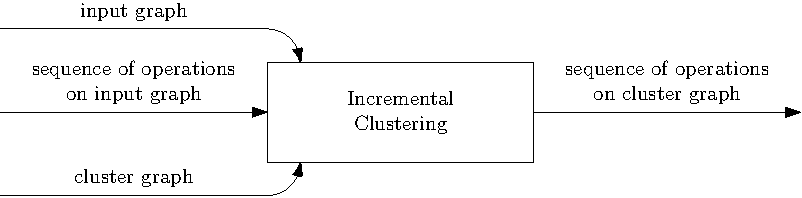
\includegraphics[width=0.8\textwidth]{Resources/DynamicPipeline-IncrementalClustering.pdf}
	\caption{Input and output of the incremental clustering phase.}
	\label{fig:dynamic-pipeline-incremental-transformation}
\end{figure}

The cluster graph of the previous version of the input graph is needed because the output sequence is tailored to a specific cluster graph. It has to be specified as input rather than being part of the output because we want to continue propagating the changes through the pipeline and apply it to a product of a non-incremental phase eventually. If we didn't specify these products as input to the incremental phases, the sequence of operations might not be compatible with the products of the non-incremental phases.

We assume that in concrete implementations, the cluster graph preserves enough information about the input graph to allow for incremental clustering. For example, the cluster graph might keep track of which vertices of input graph its clusters contain.
\todo{Or do we want to formalize that with explicit mathematical definitions of cluster graph etc.?}

The following operations on the cluster graph can be output and are sufficient to turn any cluster graph into a different one:
%
\begin{itemize}
	\setlength\itemsep{-0.5em}
	\item change a vertex' weight
	\item change an edge's weight
	\item add a vertex with arbitrary weight and edge weights to existing vertices
	\item remove a vertex
\end{itemize}
%
Note that because the cluster graph is a complete graph, we are not allowed to add or remove individual edges and adding a new vertex to the cluster graph implicitly adds edges to all existing vertices.

\clearpage
\section{Incremental Filtering and Embedding}
\label{sect:incremental-filtering-and-embedding}

The incremental filtering and embedding phase continues propagating the changes and translates changes of the cluster graph to changes of its filtered graph embedding: it takes a cluster graph, a sequence of operations to be applied to the cluster graph, and the embedded filtered graph of the cluster graph and outputs a sequence of operations that, when applied to the embedded filter graph, makes it an embedded filter graph of the cluster graph with the operations applied.

\begin{figure}[H]
	\centering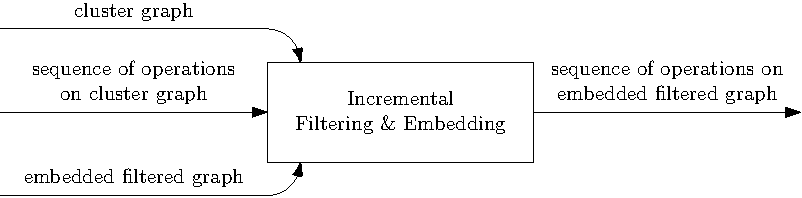
\includegraphics[width=0.9\textwidth]{Resources/DynamicPipeline-IncrementalFilteringAndEmbedding.pdf}
	\caption{Input and output of the incremental filtering and embedding phase.}
	\label{fig:dynamic-pipeline-incremental-filtering-and-embedding}
\end{figure}

The pipeline supports the following operations:
%Supported operations on embedded filtered graph:
%
\begin{itemize}
	\item \textbf{Change vertex or edge weight:}
	\item \textbf{Add vertex in an internal face:} with arbitrary weight inside an inner face (and connect it to the three vertices of the triangle)
	\item \textbf{Add vertex in outer face:} adjacent to 2 or more vertices on outer face that lie on simple path
	\item \textbf{Remove internal vertex:} of degree 3
	\item \textbf{Add edge on outer face:}
	\item \textbf{Remove edge on outer face:} without violating 2-connectedness and internal triangulatedness
	\item \textbf{Flip internal edge:}
\end{itemize}

\clearpage
\section{Incremental Transformation to Dual}
\label{sect:incremental-transformation-to-dual}

\lipsum

\begin{figure}[H]
	\centering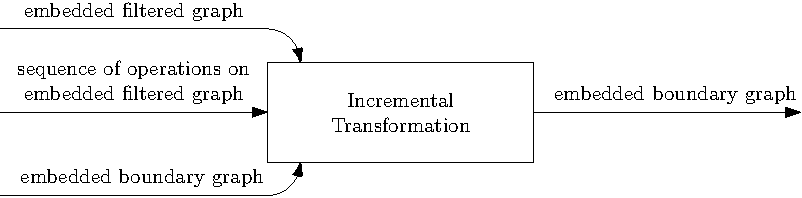
\includegraphics[width=0.9\textwidth]{Resources/DynamicPipeline-IncrementalTransformation.pdf}
	\caption{Input and output of the incremental transformation phase.}
	\label{fig:dynamic-pipeline-incremental-transformation}
\end{figure}

Supported operations translate 1 to 1 from embedded filtered graph:
%
\begin{itemize}
	\item xxx. replace vertex with face. replace edge with adjacency.
\end{itemize}

